

\tikzset{every picture/.style={line width=0.75pt}} %set default line width to 0.75pt        

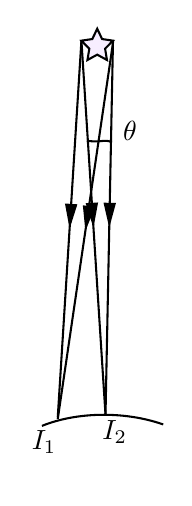
\begin{tikzpicture}[x=0.75pt,y=0.75pt,yscale=-1,xscale=1]
%uncomment if require: \path (0,300); %set diagram left start at 0, and has height of 300

%Shape: Star [id:dp7993730556190444] 
\draw  [fill={rgb, 255:red, 144; green, 19; blue, 254 }  ,fill opacity=0.07 ] (115,22.33) -- (117.35,27.3) -- (122.61,28.09) -- (118.8,31.95) -- (119.7,37.41) -- (115,34.83) -- (110.3,37.41) -- (111.2,31.95) -- (107.39,28.09) -- (112.65,27.3) -- cycle ;
%Straight Lines [id:da6010958544087177] 
\draw    (107.39,28.09) -- (119,208.33) ;
\draw [shift={(113.2,118.21)}, rotate = 266.31] [fill={rgb, 255:red, 0; green, 0; blue, 0 }  ][line width=0.08]  [draw opacity=0] (12,-3) -- (0,0) -- (12,3) -- cycle    ;
%Straight Lines [id:da5792212007108453] 
\draw    (122.61,28.09) -- (119,208.33) ;
\draw [shift={(120.8,118.21)}, rotate = 271.15] [fill={rgb, 255:red, 0; green, 0; blue, 0 }  ][line width=0.08]  [draw opacity=0] (12,-3) -- (0,0) -- (12,3) -- cycle    ;
%Shape: Arc [id:dp02266441256288565] 
\draw  [draw opacity=0] (88.36,213.69) .. controls (97.39,210.04) and (108.63,208.04) .. (120.75,208.37) .. controls (130.27,208.63) and (139.16,210.3) .. (146.81,213) -- (119.93,238.36) -- cycle ; \draw   (88.36,213.69) .. controls (97.39,210.04) and (108.63,208.04) .. (120.75,208.37) .. controls (130.27,208.63) and (139.16,210.3) .. (146.81,213) ;
%Curve Lines [id:da2800220853905422] 
\draw    (110,76.33) .. controls (118,77.33) and (118,75.33) .. (122,77) ;
%Straight Lines [id:da7563818948167416] 
\draw    (107.39,28.09) -- (96,209.33) ;
\draw [shift={(101.7,118.71)}, rotate = 273.6] [fill={rgb, 255:red, 0; green, 0; blue, 0 }  ][line width=0.08]  [draw opacity=0] (12,-3) -- (0,0) -- (12,3) -- cycle    ;
%Straight Lines [id:da6535572732710992] 
\draw    (122.61,29.09) -- (96,210.33) ;
\draw [shift={(109.3,119.71)}, rotate = 278.35] [fill={rgb, 255:red, 0; green, 0; blue, 0 }  ][line width=0.08]  [draw opacity=0] (12,-3) -- (0,0) -- (12,3) -- cycle    ;

% Text Node
\draw (126,65.4) node [anchor=north west][inner sep=0.75pt]    {$\theta $};
% Text Node
\draw (82,214.4) node [anchor=north west][inner sep=0.75pt]    {$I_{1}$};
% Text Node
\draw (116,209.4) node [anchor=north west][inner sep=0.75pt]    {$I_{2}$};


\end{tikzpicture}
